\section{Clasificación}

El aprendizaje supervisado es una técnica donde un modelo aprende a partir de datos etiquetados. En este proyecto se desarrolló un modelo
de clasificación supervisada utilizando el dataset proporcionado con el objetivo de predecir la variable \texttt{ESTATUS\_VICTIMA}.

El objetivo principal fue construir un modelo capaz de identificar patrones en los datos y realizar predicciones sobre el estatus de
una víctima utilizando diferentes variables del dataset.

Además de entrenar el modelo, también se realizó:

\begin{itemize}
    \item División de entrenamiento y prueba.
    \item Evaluación mediante métricas de desempeño.
    \item Análisis de variables relevantes.
    \item Identificación de posibles sesgos en los datos.
    \item Relación de las métricas con escenarios reales.
\end{itemize}

\subsection{Descripción del problema}

El problema consiste realizar una clasificación multiclase, ya que la variable objetivo \texttt{ESTATUS\_VICTIMA} puede contener diferentes categorías.

Entre las posibles clases se encuentran:

\begin{itemize}
    \item DESAPARECIDA
    \item NO LOCALIZADA
    \item CONFIDENCIAL
\end{itemize}

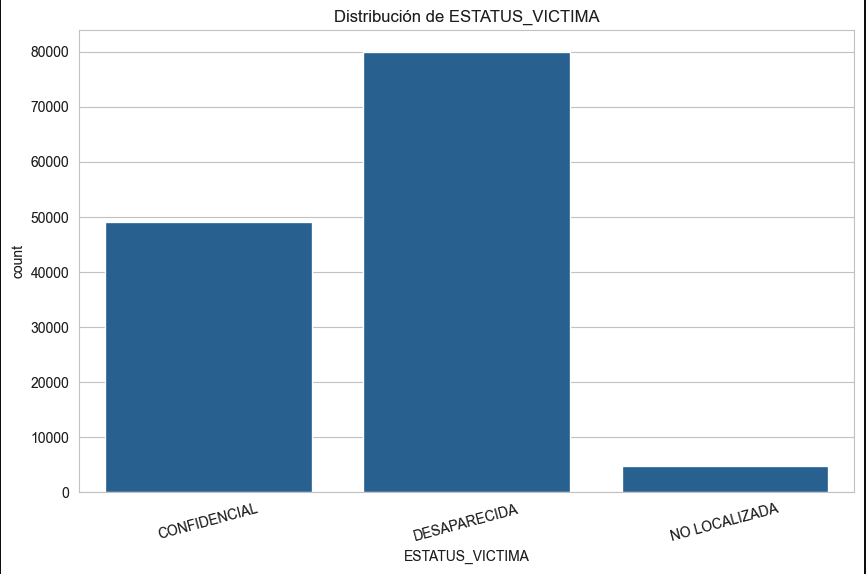
\includegraphics[width=0.7\textwidth]{imagenes/estatus_victima.png}

El propósito del modelo es aprender las relaciones entre las variables predictoras y la variable objetivo para posteriormente realizar predicciones
automáticas.

\subsection{Preparación de los datos}

Antes del entrenamiento del modelo fue necesario realizar una etapa de limpieza y preparación de datos.

Se realizaron las siguientes transformaciones:

\begin{itemize}
    \item Eliminación de identificadores únicos como \texttt{ID\_VICTIMA}, ya que no aportan información predictiva.
    \item Conversión de variables de fecha a formato datetime.
    \item Codificación de variables categóricas utilizando \texttt{LabelEncoder}.
    \item Manejo de valores faltantes mediante imputación.
\end{itemize}

Para evitar problemas durante el entrenamiento:

\begin{itemize}
    \item Las variables categóricas fueron rellenadas con el valor \texttt{DESCONOCIDO}.
    \item Las variables numéricas fueron rellenadas con la mediana.
\end{itemize}

Esta estrategia ayuda a conservar información sin eliminar registros completos.

\begin{itemize}
    \item 80\% de datos para entrenamiento.
    \item 20\% de datos para prueba.
\end{itemize}

La división se realizó utilizando \texttt{train\_test\_split()} de Scikit-learn.

Luego, se utilizó muestreo estratificado mediante el parámetro $stratify = y_encoded$, lo que garantiza que la
proporción de clases se mantenga tanto en entrenamiento como en prueba.

Otra cosa a notar es que el dataset presenta desbalance de clases. Algunas categorías tienen muchos más registros que otras.
Sin muestreo estratificado podrían ocurrir problemas como:

\begin{itemize}
    \item Clases mal representadas.
    \item Evaluaciones poco confiables.
    \item Sesgo hacia la clase mayoritaria.
\end{itemize}

Por ello, el muestreo estratificado es importante para mantener una representación adecuada de todas las clases.

\subsection{\texttt{Random Forest Classifier}}

El modelo seleccionado para la clasificación fue el \texttt{Random Forest Classifier}, un algoritmo de aprendizaje supervisado basado en árboles de decisión.
Se eligió este modelo debido a sus múltiples ventajas:

\begin{enumerate}
    \item Maneja adecuadamente variables categóricas y relaciones no lineales.
    \item Es robusto ante ruido y datos incompletos.
    \item Reduce el sobreajuste en comparación con un árbol de decisión simple.
    \item Funciona bien en datasets desbalanceados utilizando \texttt{class\_weight='balanced'}.
    \item Permite analizar la importancia de variables.
    \item Ofrece un buen desempeño sin requerir ajustes extremadamente complejos.
\end{enumerate}

Para evaluar el modelo se utilizaron las siguientes métricas y diagramas:

\subsubsection{Accuracy}

Para medir el porcentaje total de predicciones correctas y evaluar el desempeño general del modelo. Aunque proporciona una métrica
sencilla de interpretar, en datasets desbalanceados puede resultar engañosa, ya que un modelo podría predecir siempre la clase
mayoritaria y aún así obtener un accuracy alto.

\[Accuracy = \frac{TP + TN}{TP + TN + FP + FN}\]

\begin{itemize}
    \item TP = Verdaderos positivos.
    \item TN = Verdaderos negativos.
    \item FP = Falsos positivos.
    \item FN = Falsos negativos.
\end{itemize}

Un valor alto de Accuracy indica que el modelo clasifica correctamente una gran proporción de registros. Sin embargo, debido al
desbalance de clases del dataset, este resultado debe interpretarse con cuidado.

Por ejemplo, si la mayoría de los registros pertenecen a una sola clase, el modelo podría obtener un Accuracy relativamente alto incluso
si tiene dificultades para identificar correctamente las clases minoritarias.

\subsubsection{Precision}

$$Precision = \frac{TP}{TP + FP}$$

Para medir qué tan confiables son las predicciones positivas. Es importante cuando los falsos positivos generan consecuencias negativas.
En un contexto real, clasificar incorrectamente un caso podría provocar:

\begin{itemize}
    \item Uso innecesario de recursos.
    \item Investigaciones equivocadas.
    \item Información incorrecta.
\end{itemize}

Un valor alto de precisión significa que cuando el modelo predice una determinada categoría, generalmente tiene razón. En un escenario real
esto es importante porque:

\begin{itemize}
    \item Reduce falsas alarmas.
    \item Evita investigaciones innecesarias.
    \item Disminuye el uso incorrecto de recursos.
\end{itemize}

Si la precisión fuera baja, el modelo estaría clasificando incorrectamente muchos registros.

\subsubsection{Recall}

$$Recall = \frac{TP}{TP + FN}$$

En problemas relacionados con personas desaparecidas es importante minimizar los falsos negativos. Un falso negativo significa
que el modelo no detectó correctamente un caso real. Esto puede implicar:

\begin{itemize}
    \item Casos relevantes ignorados.
    \item Retrasos en procesos de búsqueda.
    \item Información incorrecta para la toma de decisiones.
\end{itemize}

Un recall alto significa que el modelo logra identificar la mayoría de los casos verdaderos. Si el Recall fuera bajo, significaría que
el modelo está dejando pasar demasiados casos reales.

\subsubsection{F1-Score}

$$F1-Score = 2 \cdot \frac{Precision \cdot Recall}{Precision + Recall}$$

El dataset presenta un desbalance de clases, por lo que el F1-Score es una métrica más adecuada para evaluar el desempeño del modelo, pues:
\begin{itemize}
    \item Detecta correctamente casos positivos.
    \item Evita demasiadas falsas alarmas.
\end{itemize}

Por ello es una métrica más robusta que Accuracy en escenarios desbalanceados. Incluso, es un resumen del equilibrio entre Precision y Recall,
lo que permite evaluar el desempeño del modelo de manera más completa.

\subsubsection{Matriz de confusión}

La matriz de confusión es una herramienta visual que muestra el desempeño del modelo en términos de verdaderos positivos, falsos positivos,
verdaderos negativos y falsos negativos para cada clase. Permite identificar patrones de error específicos, como por ejemplo:

\begin{itemize}
    \item Qué clases son clasificadas correctamente.
    \item Qué clases presentan más errores.
    \item Cuáles categorías son confundidas con mayor frecuencia.
\end{itemize}

Esto ayuda a identificar posibles problemas del modelo y entender mejor el comportamiento de las predicciones.

\subsubsection{Importancia de variables}

Una ventaja de Random Forest es que permite analizar la importancia de las variables. Las variables con mayor importancia son aquellas
que más contribuyen a las decisiones del modelo. Entre las variables potencialmente relevantes se encuentran:

\begin{itemize}
    \item Sexo.
    \item Entidad federativa.
    \item Edad o año de nacimiento.
    \item Fecha de desaparición.
    \item Año de registro.
\end{itemize}

Estas variables pueden contener patrones útiles para la clasificación.

\subsection{Resultados}

\begin{lstlisting}[language=Python, caption=Resultados del modelo]
Accuracy : 0.9735
Precision : 0.9709
Recall : 0.9735
F1-score : 0.9718
               precision    recall  f1-score   support

 CONFIDENCIAL       1.00      1.00      1.00      9830
 DESAPARECIDA       0.97      0.99      0.98     15977
NO LOCALIZADA       0.68      0.51      0.58       971

     accuracy                           0.97     26778
    macro avg       0.88      0.83      0.85     26778
 weighted avg       0.97      0.97      0.97     26778
 \end{lstlisting}

 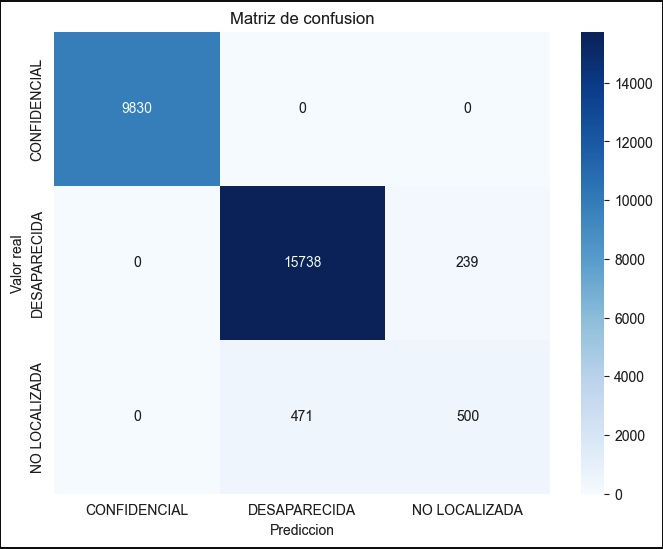
\includegraphics[width=0.7\textwidth]{imagenes/matriz_confusion.png}

 \begin{itemize}
        \item El modelo muestra un buen desempeño general con un Accuracy del 97.35\%. Pero puede ser engañoso debido al desbalance de clases.
        \item La clase CONFIDENCIAL tiene una precisión y recall perfectos, lo que indica que el modelo clasifica correctamente todos los casos de esta categoría.
        \item La clase DESAPARECIDA también tiene un desempeño excelente con una precisión del 97\% y un recall del 99\%.
        \item Sin embargo, la clase NO LOCALIZADA presenta un desempeño más bajo, con una precisión del 68\% y un recall del 51\%, lo que indica que el modelo tiene
        dificultades para identificar correctamente esta categoría.
        \item El F1-score general es alto, pero es importante considerar, nuevamente, el desbalance de clases al interpretar estos resultados.
        \item La matriz de confusión muestra que la mayoría de los errores ocurren en la clase NO LOCALIZADA, lo que sugiere que el modelo tiene
        dificultades para distinguir esta categoría de las otra. (lo cual coincide con el desempeño bajo mencionado anteriormente).
 \end{itemize}

 A pesar de estas limitaciones, el modelo proporciona una aproximación útil para la clasificación de la variable \texttt{ESTATUS\_VICTIMA}.

\begin{tcolorbox}[title=Nota]
El cuaderno de Jupyter con el código completo del modelo de clasificación se encuentra disponible en el repositorio de GitHub del proyecto.
o de manera directa en \href{https://github.com/wallsified/AyMdD_2026-2/blob/main/Tarea%203/Tarea3.ipynb}{este enlace}.
\end{tcolorbox}